% This file was created by matlab2tikz.
%
%The latest updates can be retrieved from
%  http://www.mathworks.com/matlabcentral/fileexchange/22022-matlab2tikz-matlab2tikz
%where you can also make suggestions and rate matlab2tikz.
%
\definecolor{mycolor1}{rgb}{1.00000,0.00000,1.00000}%
%
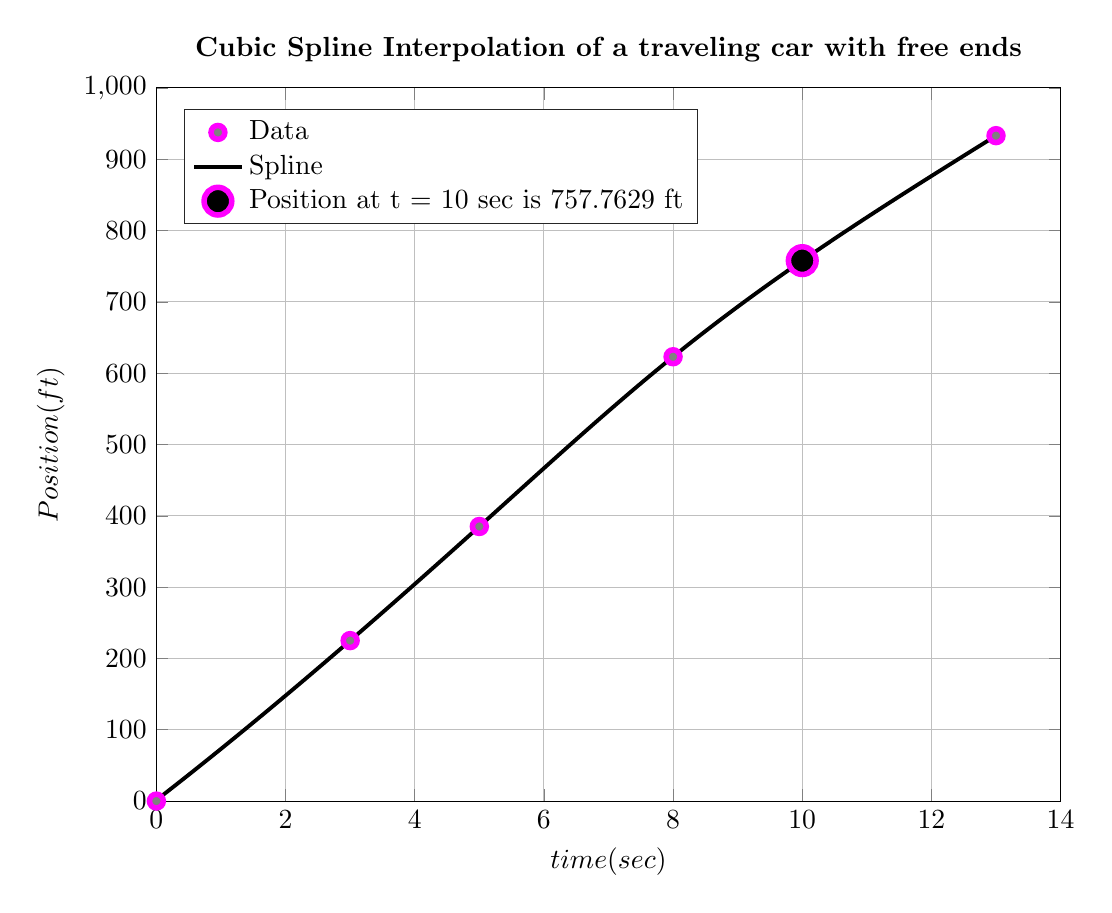
\begin{tikzpicture}

\begin{axis}[%
width=4.521in,
height=3.566in,
at={(0.758in,0.481in)},
scale only axis,
xmin=0,
xmax=14,
xlabel style={font=\bfseries},
xlabel={$time (sec)$},
xmajorgrids,
ymin=0,
ymax=1000,
ylabel style={font=\bfseries},
ylabel={$Position (ft)$},
ymajorgrids,
axis background/.style={fill=white},
title style={font=\bfseries},
title={Cubic Spline Interpolation of a traveling car with free ends},
legend style={at={(0.03,0.97)},anchor=north west,legend cell align=left,align=left,draw=white!15!black}
]
\addplot [color=mycolor1,line width=2.0pt,mark size=2.5pt,only marks,mark=*,mark options={solid,fill=gray}]
  table[row sep=crcr]{%
0	0\\
3	225\\
5	385\\
8	623\\
13	933\\
};
\addlegendentry{Data};

\addplot [color=black,solid,line width=1.4pt]
  table[row sep=crcr]{%
0	1.35390428211588\\
0.1	8.394058201664\\
0.2	15.4666965880467\\
0.3	22.5714033661553\\
0.4	29.7077624608808\\
0.5	36.8753577971148\\
0.6	44.0737732997481\\
0.7	51.3025928936723\\
0.8	58.5614005037783\\
0.9	65.8497800549576\\
1	73.1673154721014\\
1.1	80.5135906801008\\
1.2	87.8881896038471\\
1.3	95.2906961682314\\
1.4	102.720694298145\\
1.5	110.17776791848\\
1.6	117.661500954126\\
1.7	125.171477329975\\
1.8	132.707280970918\\
1.9	140.268495801847\\
2	147.854705747653\\
2.1	155.465494733226\\
2.2	163.100446683459\\
2.3	170.759145523243\\
2.4	178.441175177467\\
2.5	186.146119571025\\
2.6	193.873562628807\\
2.7	201.623088275704\\
2.8	209.394280436608\\
2.9	217.186723036409\\
3	225\\
3.1	232.833695252271\\
3.2	240.687392718113\\
3.3	248.560676322418\\
3.4	256.453129990077\\
3.5	264.364337645981\\
3.6	272.293883215022\\
3.7	280.24135062209\\
3.8	288.206323792077\\
3.9	296.188386649874\\
4	304.187123120372\\
4.1	312.202117128464\\
4.2	320.232952599038\\
4.3	328.279213456988\\
4.4	336.340483627204\\
4.5	344.416347034577\\
4.6	352.506387604\\
4.7	360.610189260362\\
4.8	368.727335928555\\
4.9	376.857411533471\\
5	385\\
5.1	393.154313682586\\
5.2	401.318078653877\\
5.3	409.488649416075\\
5.4	417.66338047138\\
5.5	425.839626321994\\
5.6	434.014741470117\\
5.7	442.186080417949\\
5.8	450.350997667693\\
5.9	458.506847721548\\
6	466.650985081716\\
6.1	474.780764250397\\
6.2	482.893539729792\\
6.3	490.986666022102\\
6.4	499.057497629528\\
6.5	507.103389054271\\
6.6	515.121694798531\\
6.7	523.10976936451\\
6.8	531.064967254408\\
6.9	538.984642970426\\
7	546.866151014766\\
7.1	554.706845889627\\
7.2	562.50408209721\\
7.3	570.255214139718\\
7.4	577.95759651935\\
7.5	585.608583738307\\
7.6	593.20553029879\\
7.7	600.745790703\\
7.8	608.226719453138\\
7.9	615.645671051404\\
8	623\\
8.1	630.287725944584\\
8.2	637.509529104648\\
8.3	644.666754843142\\
8.4	651.760748523013\\
8.5	658.792855507213\\
8.6	665.76442115869\\
8.7	672.676790840394\\
8.8	679.531309915274\\
8.9	686.329323746279\\
9	693.072177696359\\
9.1	699.761217128464\\
9.2	706.397787405542\\
9.3	712.983233890543\\
9.4	719.518901946416\\
9.5	726.006136936112\\
9.6	732.446284222578\\
9.7	738.840689168766\\
9.8	745.190697137623\\
9.9	751.4976534921\\
10	757.762903595145\\
10.1	763.987792809709\\
10.2	770.17366649874\\
10.3	776.321870025189\\
10.4	782.433748752004\\
10.5	788.510648042134\\
10.6	794.55391325853\\
10.7	800.56488976414\\
10.8	806.544922921914\\
10.9	812.495358094802\\
11	818.417540645752\\
11.1	824.312815937715\\
11.2	830.182529333639\\
11.3	836.028026196474\\
11.4	841.850651889169\\
11.5	847.651751774674\\
11.6	853.432671215938\\
11.7	859.19475557591\\
11.8	864.939350217541\\
11.9	870.667800503778\\
12	876.381451797573\\
12.1	882.081649461873\\
12.2	887.769738859629\\
12.3	893.44706535379\\
12.4	899.114974307305\\
12.5	904.774811083124\\
12.6	910.427921044195\\
12.7	916.075649553469\\
12.8	921.719341973895\\
12.9	927.360343668422\\
13	933\\
};
\addlegendentry{Spline};

\addplot [color=mycolor1,line width=2.0pt,mark size=5.0pt,only marks,mark=*,mark options={solid,fill=black}]
  table[row sep=crcr]{%
10	757.762903595145\\
};
\addlegendentry{Position at t = 10 sec is 757.7629 ft};

\end{axis}
\end{tikzpicture}%